% задание и сама лабораторная работа
\newpage
\section*{Задание}
\addcontentsline{toc}{section}{\tocsecindent{Задание}}
\Large{Лабораторная работа №1}\\

\large{Представить следующие списки в виде списочных ячеек:}\\
\\
1) '(open close halph) \hspace{5cm}4) '((TOOL) (call))\\
2) '((open1) (close2) (halph3)) \hspace{3.4cm}5) '((TOOL1) ((call2)) ((sell)))\\
3) '((one) for all (and(me(for you)))) \hspace{2.3cm}6) '(((TOOL) (call)) ((sell)))\\


\begin{minipage}[t]{1.0\textwidth}
  \centering\raisebox{\dimexpr \topskip-\height}{%
  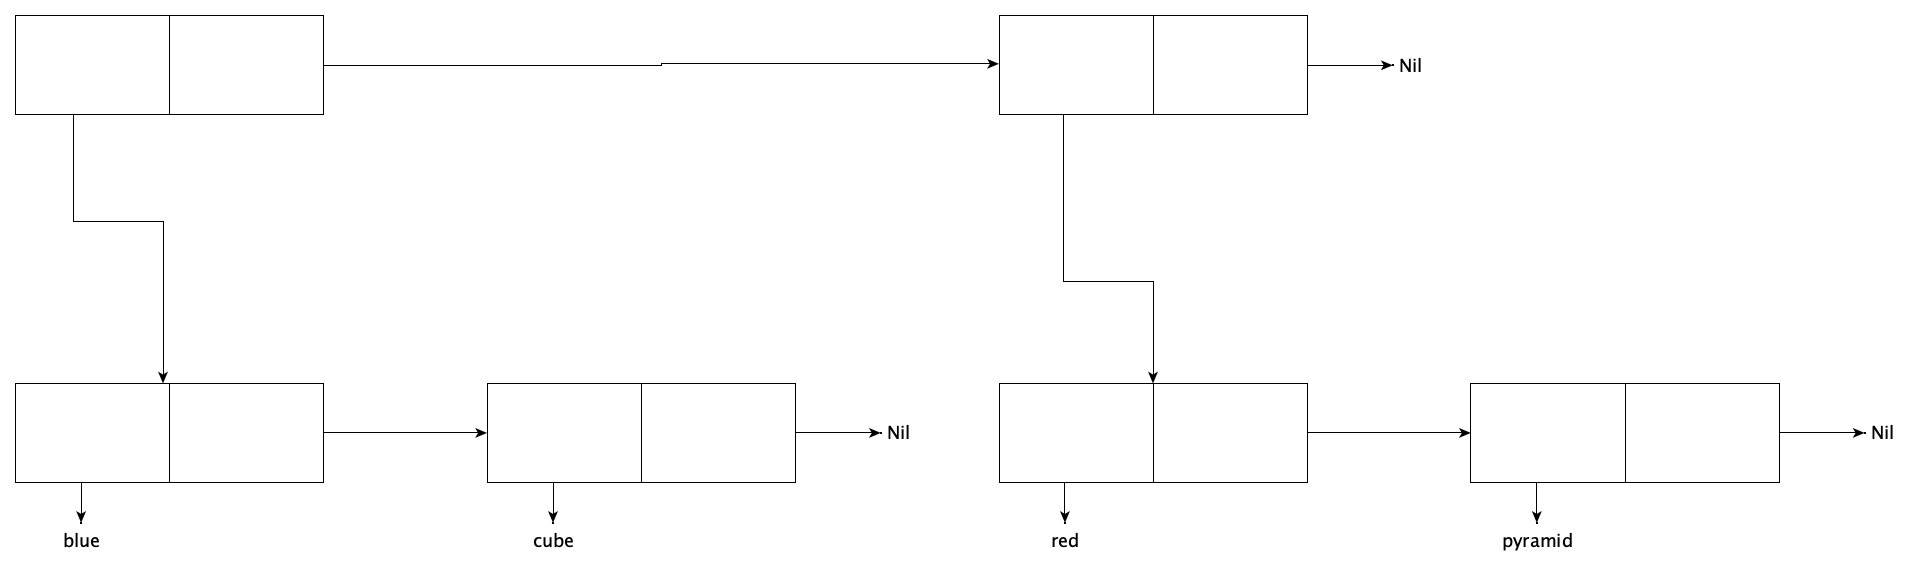
\includegraphics[width=\textwidth]{1.png}}
  \captionof{figure}{'(open close halph)}
  \label{fig1}
\end{minipage}\hfill

\begin{minipage}[t]{1.0\textwidth}
  \centering\raisebox{\dimexpr \topskip-\height}{%
  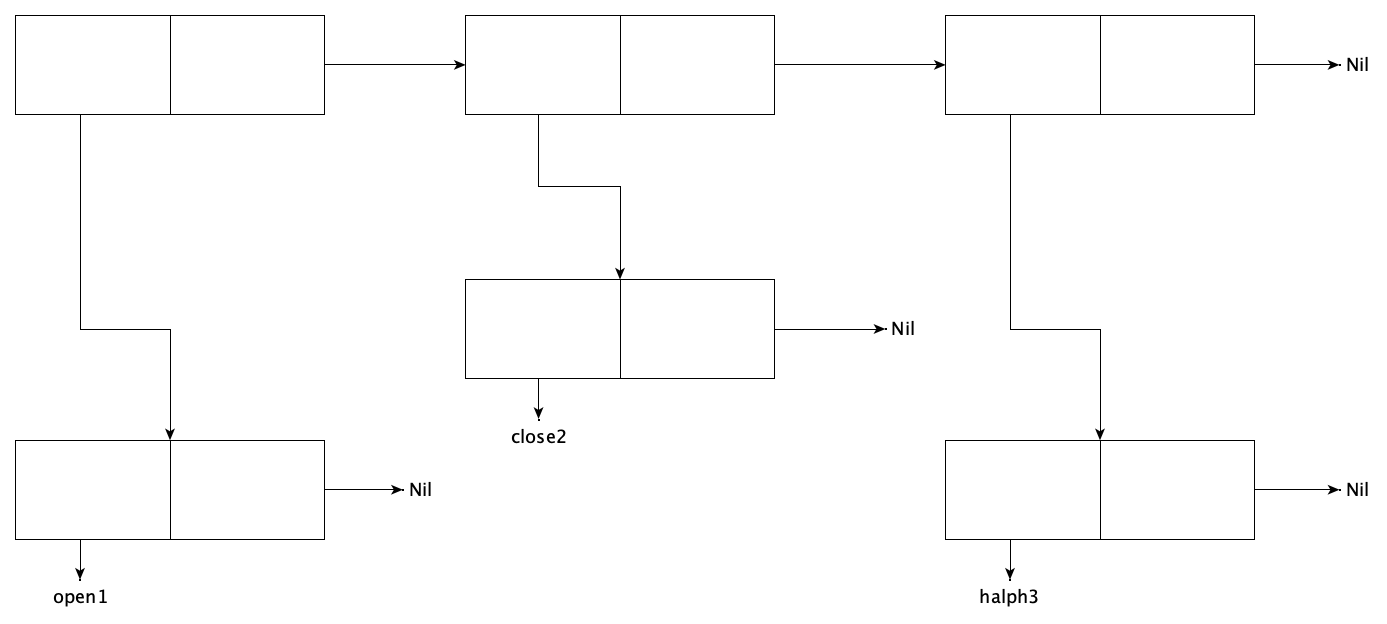
\includegraphics[width=\textwidth]{2.png}}
  \captionof{figure}{'((open1) (close2) (halph3)) }
  \label{fig2}
\end{minipage}\hfill

\begin{minipage}[t]{1.0\textwidth}
  \centering\raisebox{\dimexpr \topskip-\height}{%
  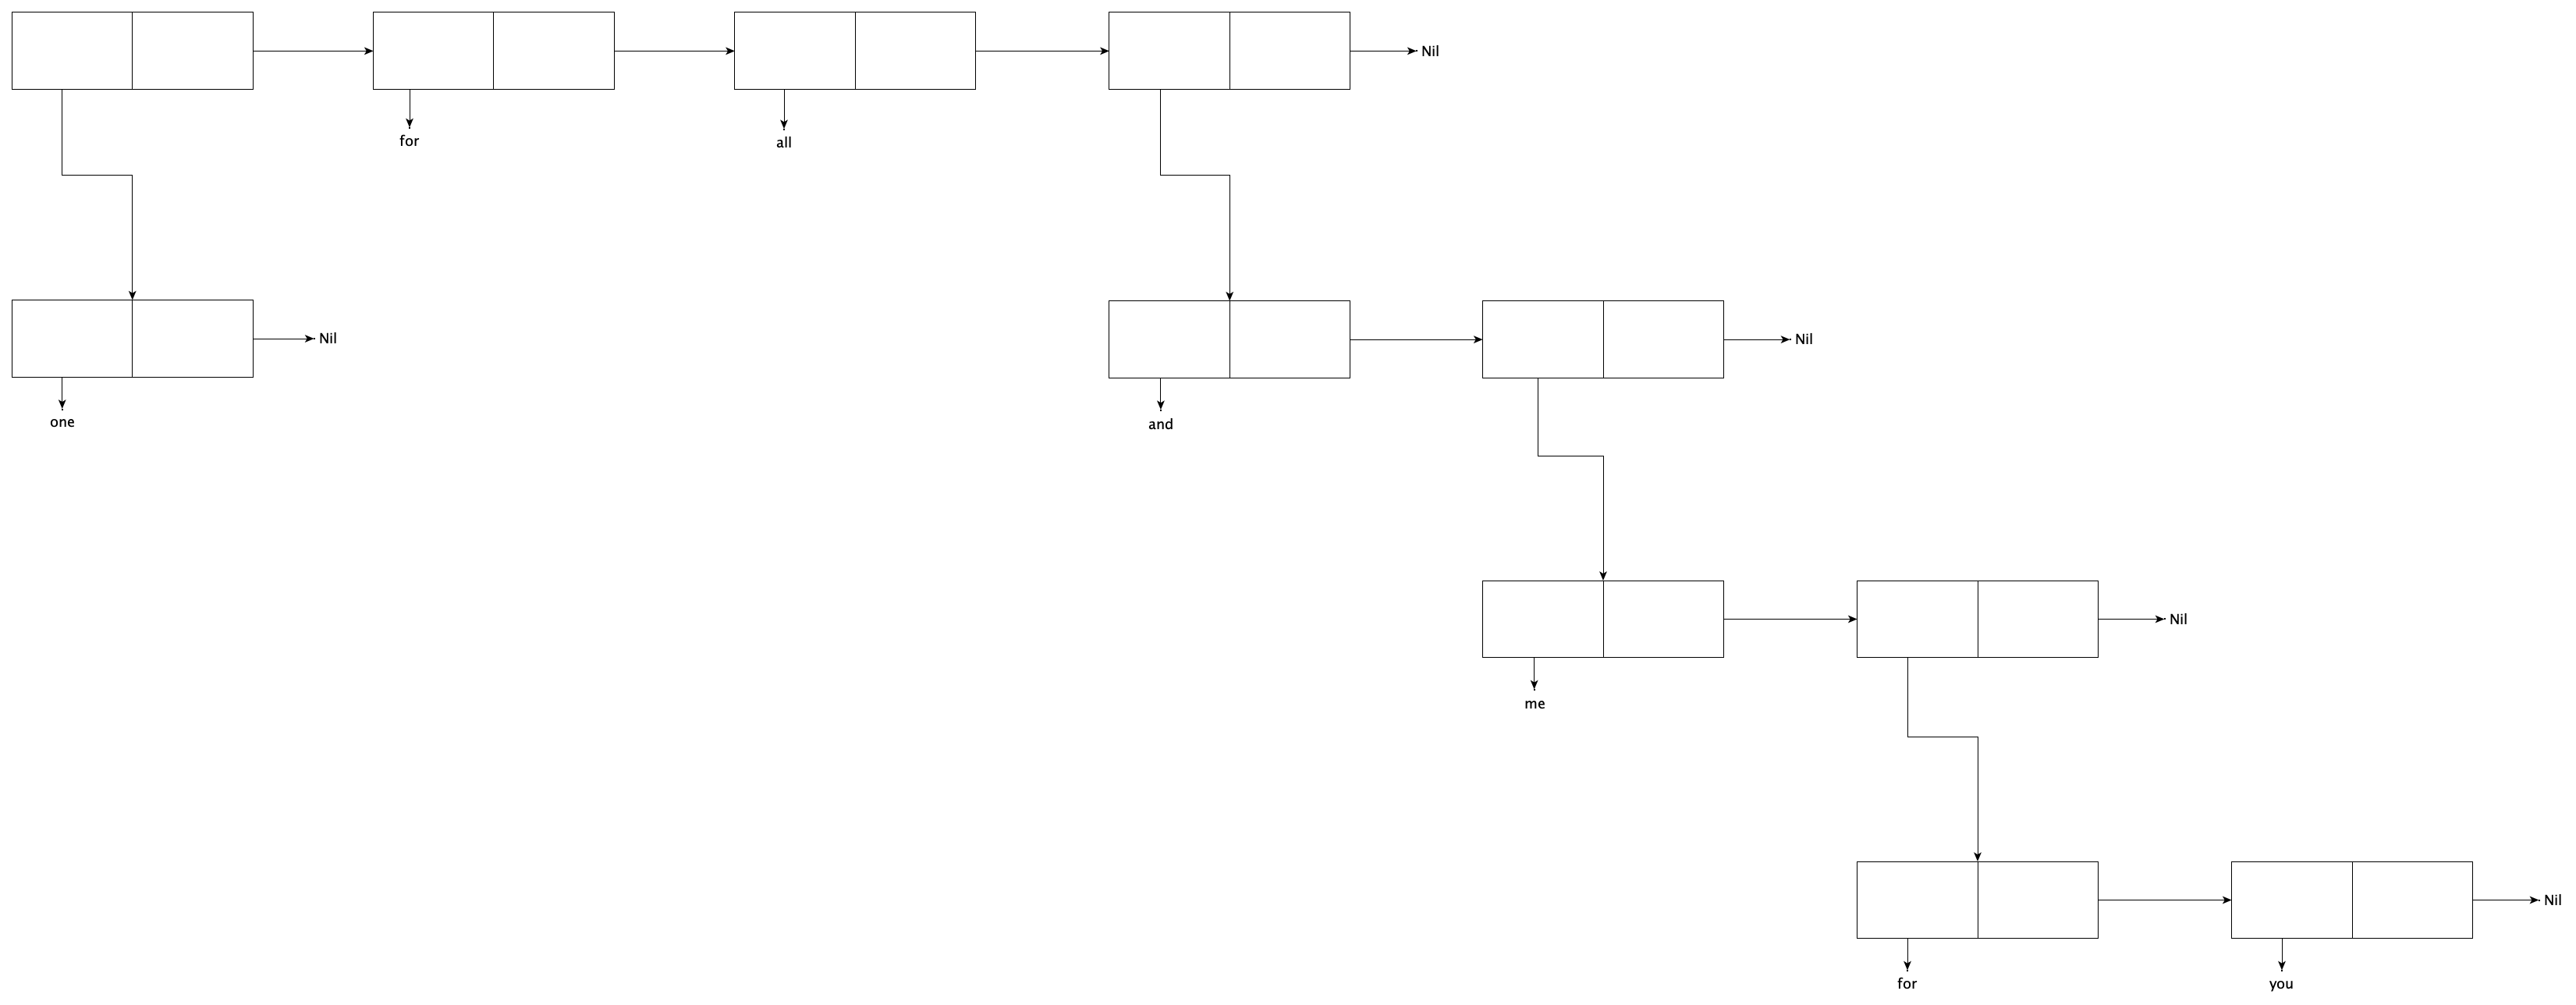
\includegraphics[width=\textwidth]{3.png}}
  \captionof{figure}{'((one) for all (and(me(for you))))}
  \label{fig3}
\end{minipage}\hfill

\begin{minipage}[t]{1.0\textwidth}
  \centering\raisebox{\dimexpr \topskip-\height}{%
  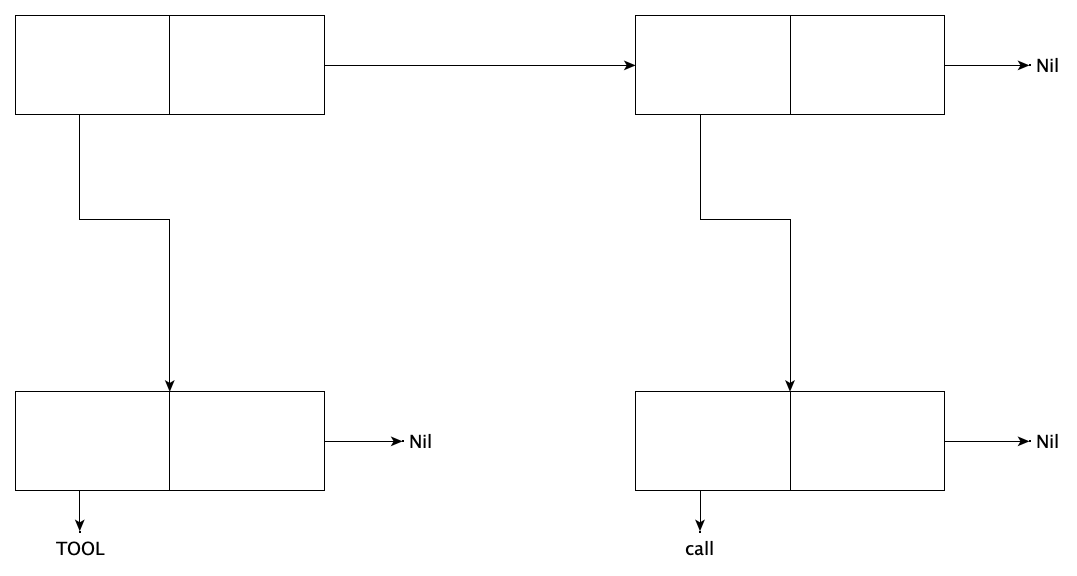
\includegraphics[width=\textwidth]{4.png}}
  \captionof{figure}{'((TOOL) (call))}
  \label{fig4}
\end{minipage}\hfill

\begin{minipage}[t]{1.0\textwidth}
  \centering\raisebox{\dimexpr \topskip-\height}{%
  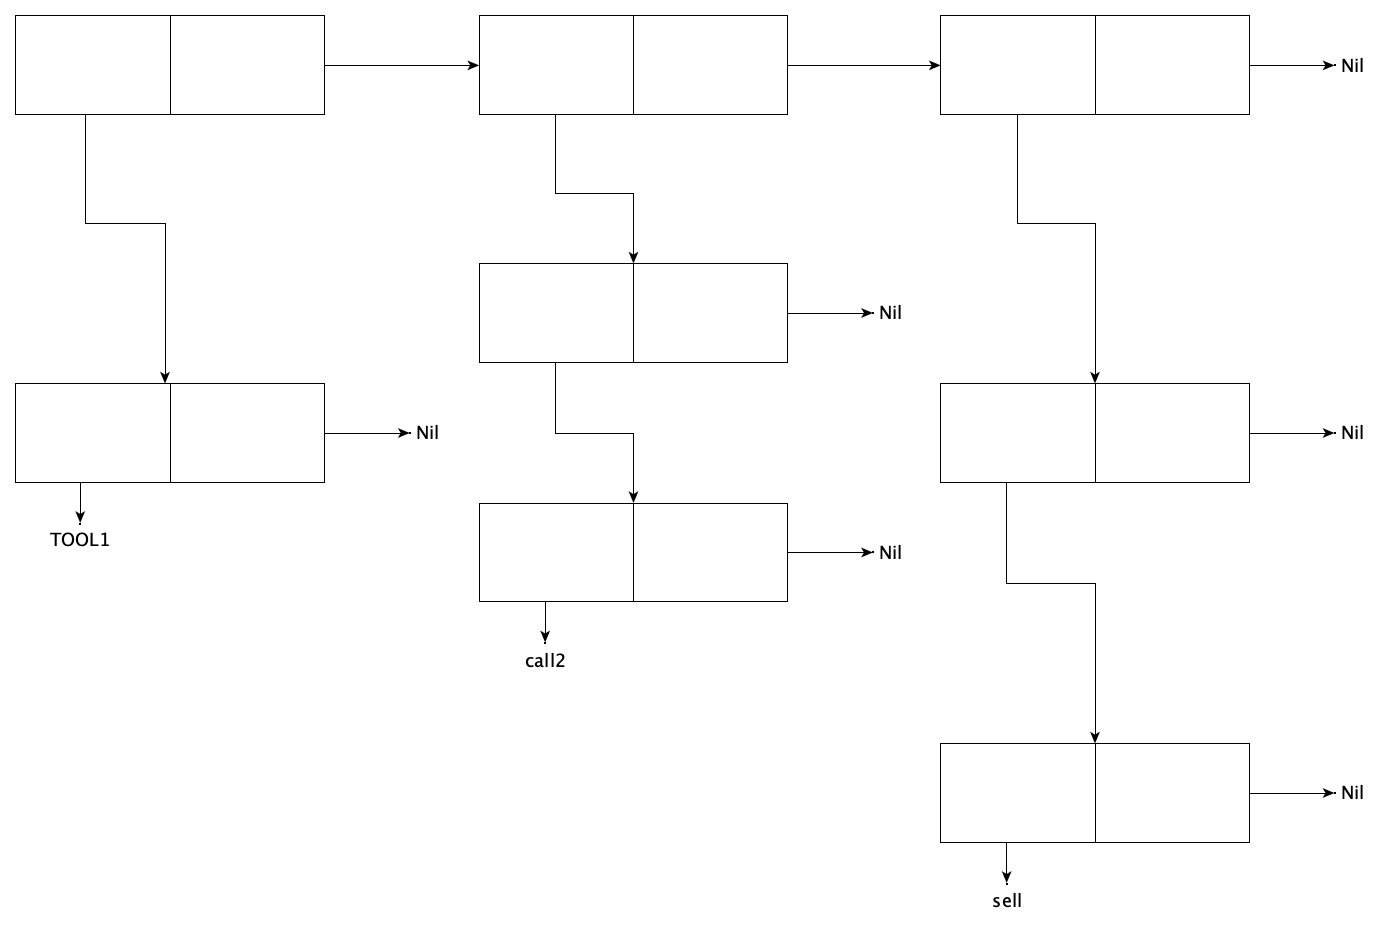
\includegraphics[width=\textwidth]{5.png}}
  \captionof{figure}{'((TOOL1) ((call2)) ((sell)))}
  \label{fig5}
\end{minipage}\hfill

\begin{minipage}[t]{1.0\textwidth}
  \centering\raisebox{\dimexpr \topskip-\height}{%
  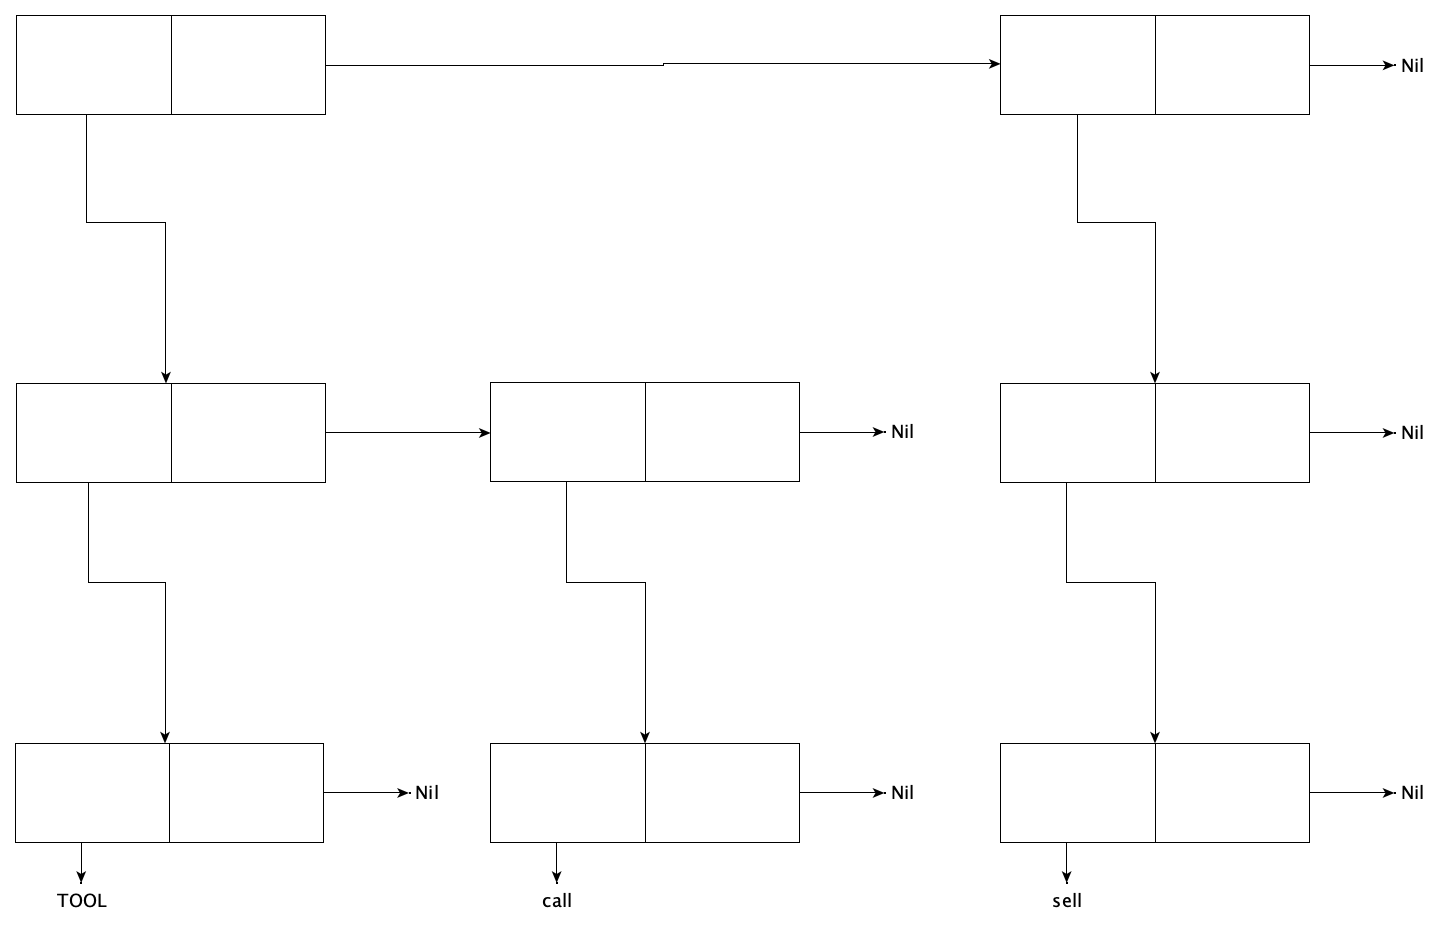
\includegraphics[width=\textwidth]{6.png}}
  \captionof{figure}{'(((TOOL) (call)) ((sell)))}
  \label{fig6}
\end{minipage}\hfill

